\section*{Appendix: Diagrams}

The following diagrams are included as submission-ready figures for the hackathon visual artifact slot and as reference figures for the whitepaper body.

\begin{figure}[h]
  \centering
  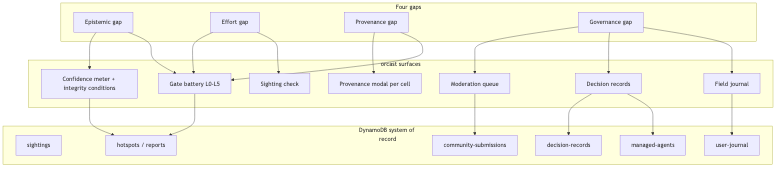
\includegraphics[width=\linewidth]{Figures/fig-1-four-gaps.png}
  \caption{%
    \textbf{The four gaps and the orcast bridge.}
    Four compounding failure modes in wildlife encounter forecasting (epistemic gap, effort gap, provenance gap, governance gap) and the orcast surfaces that address each. Each gap has at least one arrow to an operational surface; each surface writes to one or more of the nine DynamoDB tables that constitute the system of record. The architecture enforces the property that no confidence-bearing surface exists without a provenance chain and no community submission influences the model without a moderation record.%
  }
  \label{fig:four-gaps}
\end{figure}

\begin{figure}[h]
  \centering
  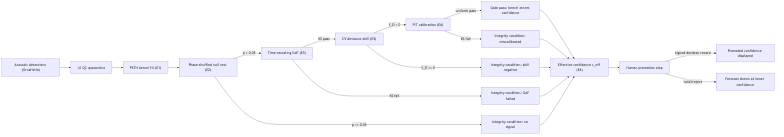
\includegraphics[width=\linewidth]{Figures/fig-2-gate-pipeline.png}
  \caption{%
    \textbf{Gate pipeline from raw detections to displayed confidence.}
    The full leveled gate battery from Level~0 QC quarantine through PSTH kernel fit (E1), phase-shuffled null test (E2), time-rescaling goodness-of-fit (E3), held-out deviance skill (E5), and PIT calibration (E6). Failing gates produce integrity conditions rather than suppressing the forecast. The human promotion step is last; effective confidence (E4) is bounded by all gate outcomes. All gate steps are present; promotion is the final node before displayed confidence.%
  }
  \label{fig:gate-pipeline}
\end{figure}

\begin{figure}[h]
  \centering
  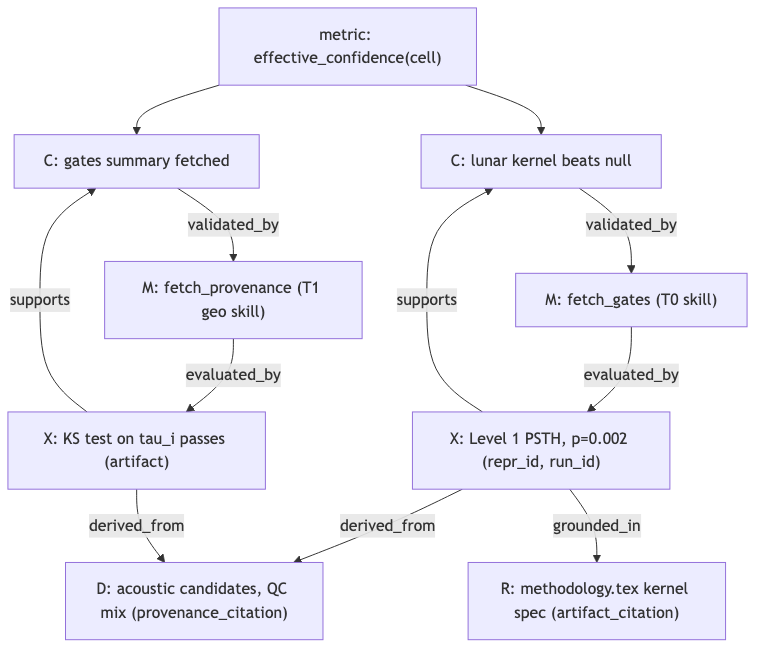
\includegraphics[width=0.88\linewidth]{Figures/fig-3-provenance-graph.png}
  \caption{%
    \textbf{Claim/method/experiment provenance graph (E8).}
    A metric node (effective confidence of a cell) traces through two claim nodes (lunar kernel beats null; gates summary fetched) to their producing method nodes (fetch\_gates T0 skill; fetch\_provenance T1 geo skill), to experiment nodes (Level~1 PSTH with artifact repr\_id/run\_id; KS test on $\tau_i$), and to data and research leaf nodes. All typed edges (validated\_by, evaluated\_by, supports, derived\_from, grounded\_in) match the contract in the methodology. This graph is rendered live by the ProvenanceGraph component from the persisted step log.%
  }
  \label{fig:provenance-graph}
\end{figure}

\begin{figure}[h]
  \centering
  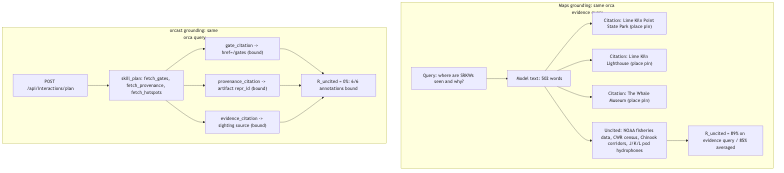
\includegraphics[width=\linewidth]{Figures/fig-4-grounding-contrast.png}
  \caption{%
    \textbf{Grounding contrast: Google Maps vs orcast on the same orca evidence query.}
    Left panel (orcast): three annotation types (gate\_citation, provenance\_citation, evidence\_citation) all bound to artifacts or hrefs; $R_\mathrm{uncited} = 0\%$. Right panel (Maps grounding): same query produces 502 words citing three place pins; NOAA fisheries data, Center for Whale Research census, Chinook salmon corridors, and J/K/L pod hydrophone data are all uncited; $R_\mathrm{uncited} = 89\%$ on the evidence query, 85\% averaged (benchmark run 2026-06-24, Gemini 3.5 Flash, Api-Revision 2026-05-20).%
  }
  \label{fig:grounding-contrast}
\end{figure}

\begin{figure}[h]
  \centering
  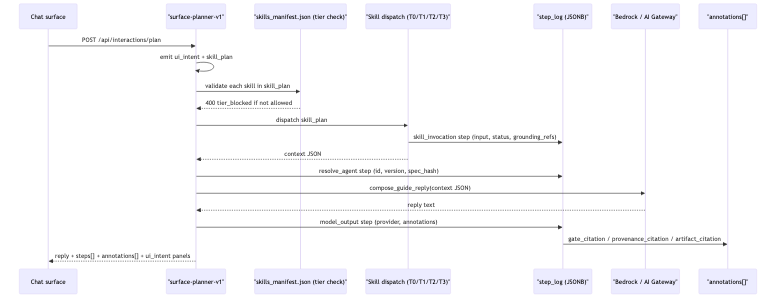
\includegraphics[width=\linewidth]{Figures/fig-5-agent-pipeline.png}
  \caption{%
    \textbf{Managed agent pipeline: plan, manifest check, dispatch, step log, annotations.}
    Sequence diagram of the surface planner interaction. The chat surface sends a request; surface-planner-v1 emits a ui\_intent and skill\_plan; each skill is validated against skills\_manifest.json before dispatch (400 tier\_blocked if not allowed); skill invocations write step log entries with input, status, and grounding references; the LLM narrates the collected context; the model\_output step records annotations (gate\_citation, provenance\_citation, artifact\_citation); the full reply with steps, annotations, and ui\_intent panels returns to the chat surface.%
  }
  \label{fig:agent-pipeline}
\end{figure}

\clearpage
\subsection*{Multi-panel figures: grounding quality benchmark}

\begin{figure}[h]
  \centering
  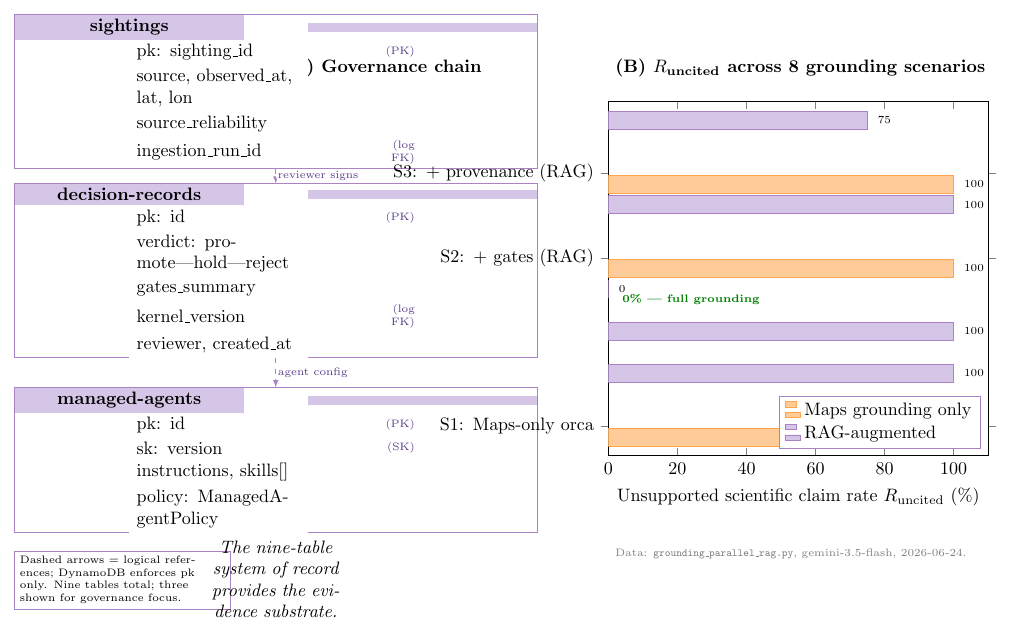
\includegraphics[width=\linewidth]{Figures/fig-mp1.png}
  \caption{%
    \textbf{Evidence-binding failure and its measurement.}
    (A) The orcast governance chain: sighting records, gate verdicts, and managed agent
    configurations linked through DynamoDB. Nine tables total; three shown for governance focus.
    The system of record provides the evidence substrate for grounding quality evaluation.
    (B) Unsupported scientific claim rate $R_\mathrm{uncited}$ across eight grounding scenarios.
    Maps-only baseline: 60--91\% uncited. Surface planner step-log (green, Scenario~4):
    $R_\mathrm{uncited} = 0\%$ --- injecting an orchestrated reasoning chain eliminates
    uncited claims entirely. Data: \texttt{grounding\_parallel\_rag.py}, gemini-3.5-flash, 2026-06-24.%
  }
  \label{fig:mp1-problem}
\end{figure}

\begin{figure}[h]
  \centering
  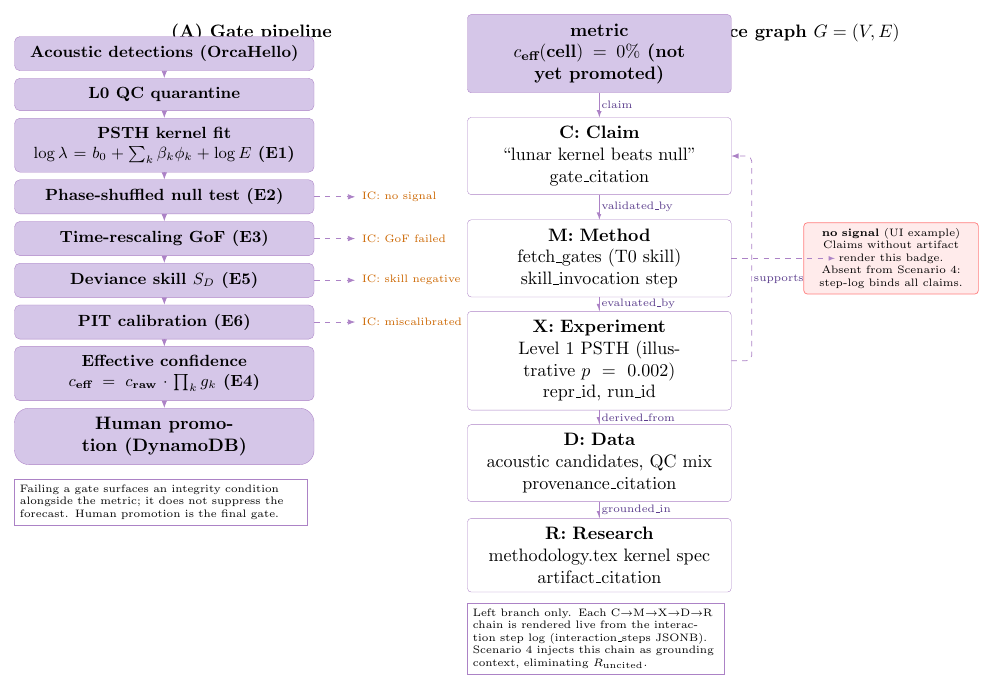
\includegraphics[width=\linewidth]{Figures/fig-mp2.png}
  \caption{%
    \textbf{The mechanism that produces 0\% uncited rate.}
    (A) Gate pipeline: acoustic detections pass through six statistical gates (E1--E6) before
    contributing to displayed confidence. Failing a gate surfaces an integrity condition rather
    than suppressing the forecast. Human promotion is the final gate.
    (B) Provenance graph $G=(V,E)$: metric root traces to Claim (C) $\to$ Method (M: skill invocation)
    $\to$ Experiment (X: artifact repr\_id/run\_id) $\to$ Data (D: provenance citation) $\to$
    Research (R: artifact citation). Claims without a bound artifact render the ``no signal'' badge.
    Scenario~4 eliminates $R_\mathrm{uncited}$ because the planner step-log binds every claim
    to an artifact reference.%
  }
  \label{fig:mp2-mechanism}
\end{figure}

\begin{figure}[h]
  \centering
  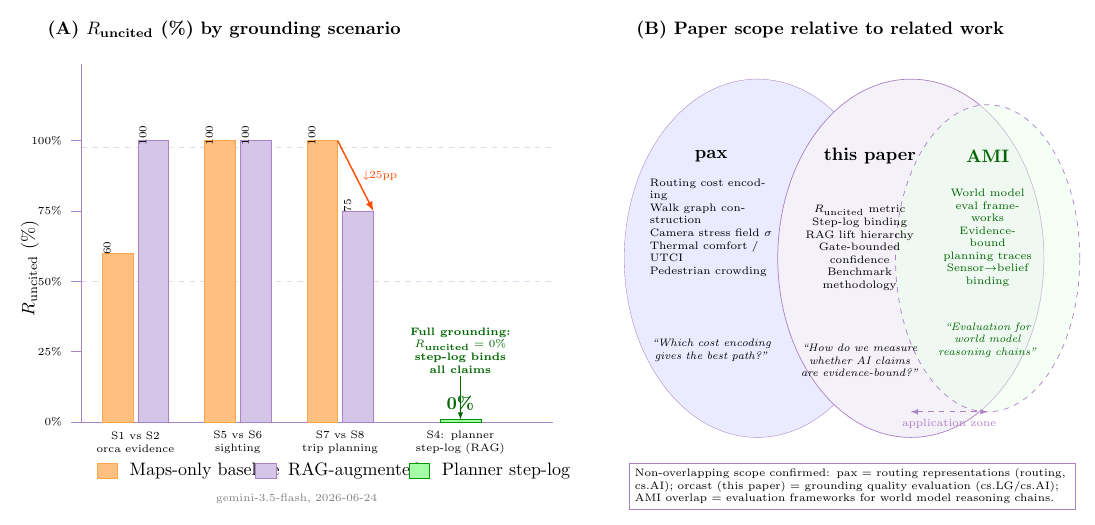
\includegraphics[width=\linewidth]{Figures/fig-mp3.png}
  \caption{%
    \textbf{Grounding quality hierarchy and paper scope.}
    (A) $R_\mathrm{uncited}$ for baseline vs RAG-augmented scenarios.
    The surface planner step-log (green, standalone at 0\%) eliminates uncited claims.
    Hotspot injection (S7$\to$S8) provides a 25 percentage point lift.
    Gate context does not reduce $R_\mathrm{uncited}$.
    (B) Paper scope relative to related work. The present paper (center) addresses
    grounding evaluation methodology --- distinct from pedestrian routing cost representations
    (pax, left) and directly applicable to world model evaluation infrastructure (AMI, right).%
  }
  \label{fig:mp3-scope}
\end{figure}
